%% LyX 2.3.6.1 created this file.  For more info, see http://www.lyx.org/.
%% Do not edit unless you really know what you are doing.
\documentclass[twocolumn,aps,prl,superscriptaddress,floatfix]{revtex4-2}
\usepackage[latin9]{inputenc}
\setcounter{secnumdepth}{3}
\usepackage{amsmath}
\usepackage{amssymb}
\usepackage{graphicx}

\makeatletter

%%%%%%%%%%%%%%%%%%%%%%%%%%%%%% LyX specific LaTeX commands.
%% Because html converters don't know tabularnewline
\providecommand{\tabularnewline}{\\}

%%%%%%%%%%%%%%%%%%%%%%%%%%%%%% User specified LaTeX commands.
%% Physical Review Letters submission
%% Spectral Dynamics of Financial Price Operators


\usepackage{amsfonts}\usepackage{dcolumn}
\usepackage{bm}
% hyperref omitted for APS submission (added by editorial system)
\usepackage{xcolor}
\usepackage{booktabs}


% Notation shortcuts
\newcommand{\K}{\mathbf{K}}
\newcommand{\phik}{\phi_k}
\newcommand{\lam}{\lambda}
\newcommand{\lamplus}{\lambda_+}
\newcommand{\dW}{d\mathcal{W}}
\newcommand{\dN}{d\mathcal{N}}
\newcommand{\tr}{\mathrm{Tr}}
\newcommand{\E}{\mathbb{E}}
\newcommand{\norm}[1]{\left\|#1\right\|_F}



\makeatother

\begin{document}
\title{Universal Spectral Phase Transitions in Financial Price Dynamics}
\author{Rafael Morgado}
\affiliation{Applied Natural Science Department, Faculty of Engineering Science
and Technology, University of Brasilia, 72444-240, Brasilia, Federal
District, Brazil}
\author{Ronne Toledo}
\affiliation{Aerospace Department, Faculty of Engineering Science and Technology,
University of Brasilia, 72444-240, Brasilia, Federal District, Brazil}
\author{Fernando A. Oliveira}
\affiliation{International Center of Physics, Institute of Physics, University
of Brasilia, 70910-900, Brasilia, Federal District, Brazil}
\date{\today}
\begin{abstract}
We demonstrate that the temporal covariance operator $\K(\tau)$ of
logarithmic price returns evolves as a matrix-valued It� process,
exhibiting universal critical exponents and spectral phase transitions.
By constructing $\K(\tau)$ via sliding Hankel embedding and decomposing
its spectrum relative to the Marchenko--Pastur (MP) bulk boundary
$\lamplus$, we identify regime changes as first-passage events of
the spectral gap $G(\tau)=\lambda_{k}(\tau)-\lamplus(\tau)$ through
zero. Empirical analysis across multiple asset classes and markets
yields two universal exponents: the diffusive scaling exponent $\beta\approx1$
of the squared Frobenius norm $\E[\|\Delta\K\|_{F}^{2}]\sim(\Delta\tau)^{\beta}$,
consistent with Markovian It� dynamics, and the inter-regime waiting-time
exponent $\alpha\approx2$, predicted analytically from first-passage
theory of one-dimensional diffusions near a regular critical point.
The bulk spectral density converges to the MP law with relative $L^{2}$
error below $4\%$. An optimal embedding dimension $L_{\text{opt}}\approx80$
and observation step $\Delta\tau_{{\rm opt}}$ emerge independently
of the observation timescale, suggesting an intrinsic finite-dimensional
structure of the market state space. These results establish a unified
spectral framework for market regime dynamics and provide the first
quantitative evidence for universality class membership of financial
phase transitions. 
\end{abstract}
\maketitle
% ============================================================


\section{Introduction}

% ============================================================

Financial price series exhibit a well-documented phenomenology that
resists simple stochastic description: persistent patterns within
regimes, abrupt structural breaks between them, volatility clustering,
and the intermittent efficacy of quantitative factors \cite{Cont2001,Bouchaud2003,Mantegna1999}.
Existing frameworks treat these features separately: GARCH models
address volatility clustering \cite{Engle1982,Bollerslev1986}, Hidden
Markov Models capture regime switching \cite{Hamilton1989}, and Random
Matrix Theory (RMT) filters noise from cross-asset covariance matrices
\cite{Laloux1999,Plerou1999}.

Here we propose a unified framework in which all these phenomena emerge
from the stochastic dynamics of a single object, the temporal covariance
operator $\K(\tau)$, constructed from the Hankel embedding of a single
scalar return series within a sliding window indexed by slow time
$\tau$. We show that $\K(\tau)$ follows a matrix It� process, that
its spectral decomposition separates structural information from universal
noise via the MP law, and that spectral phase transitions, defined
here as crossings of eigenvalues through the MP boundary, govern regime
changes.

The central result is a pair of universal exponents $(\beta,\alpha)=(1,2)$,
which we derive analytically and verify empirically across multiple
asset classes. These exponents are not free parameters, $\beta=1$
is the hallmark of Markovian diffusion, excluding long-memory processes
\cite{Beran1994}, and $\alpha=2$ is the universal first-passage
exponent of a diffusion with regular drift at a critical point \cite{Redner2001}. 

% ============================================================


\section{Construction of the Covariance Operator}

% ============================================================

Let $P(t)=\ln(S(t)/S(t-1))-\mu$ be the mean centered log-return at
discrete time $t$, where $\mu(\tau)$ is the sample mean of log--returns
within the window of length $W$ centered at $\tau$. Fix an embedding
dimension $L$ with $W>L$. At slow time $\tau$, define the Hankel
matrix 
\begin{equation}
\mathbf{X}(\tau)\in\mathbb{R}^{N\times L},\quad X_{ki}=P(\tau-W+k+i-1),\label{eq:hankel}
\end{equation}
where $N=W-L$ is the number of delay vectors. The empirical covariance
operator is 
\begin{equation}
\K(\tau)=\frac{1}{N-1}\left[\mathbf{X}(\tau)^{\top}\mathbf{X}(\tau)-N\bar{\mathbf{x}}\bar{\mathbf{x}}^{\top}\right]\in\mathbb{R}^{L\times L},\label{eq:K_def}
\end{equation}
where $\bar{\mathbf{x}}$ is the column-mean vector. Eigendecomposition
yields $\K(\tau)\phi_{k}(\tau)=\lambda_{k}(\tau)\phi_{k}(\tau)$,
with eigenvalues ordered $\lambda_{1}\geq\lambda_{2}\geq\cdots\geq\lambda_{L}$.

The MP upper boundary for the noise bulk is 
\begin{equation}
\lamplus(\tau)=\hat{\sigma}^{2}(\tau)\bigl(1+\sqrt{q}\bigr)^{2},\quad q=L/N,\label{eq:lambda_plus}
\end{equation}
where $\hat{\sigma}^{2}(\tau)$ is the empirical variance of $\mathbf{X}(\tau)$.
Eigenvalues exceeding $\lamplus$ are classified as \emph{structural
modes}; the remainder constitute the \emph{bulk}. The number of structural
modes $m(\tau)=\#\{k:\lambda_{k}(\tau)>\lamplus(\tau)\}$ defines
the instantaneous \emph{structural dimension}.

% ============================================================


\section{It� Dynamics of $\K(\tau)$}

% ============================================================

We model $\K(\tau)$ as a matrix-valued It� process: 
\begin{equation}
d\K=\mathbf{A}(\K,\tau)\,d\tau+\mathbf{B}(\K,\tau)\,d\mathcal{W}_{\tau}+\delta(\K)\,d\mathcal{N}_{\tau},\label{eq:ito_K}
\end{equation}
where $\mathbf{A}$ is a deterministic drift, $\mathbf{B}$ couples
the noise, $d\mathcal{W}$ is a matrix Wiener process, and $d\mathcal{N}$
is a Poisson process associated with large exogenous shocks.

\textbf{Diffusive scaling test.} For a matrix It� process without
the jump term, $\E[\|\K(\tau+\Delta\tau)-\K(\tau)\|_{F}^{2}]\sim(\Delta\tau)^{\beta}$
with $\beta=1$. We estimate $\beta$ empirically by subsampling $\K$
at lags $\Delta\tau\in\{1,2,4,8,16\}\times\Delta\tau_{0}$, where
$\Delta\tau_{0}$is observation step, and fitting a log-log regression.
Systematic deviation from $\beta=1$ would falsify the It� hypothesis.

\textbf{Fluctuation--dissipation balance.} Applying the It� rule
to the Frobenius energy $\mathcal{E}=\tr(\K^{\top}\K)=[\K:\K]$: 
\begin{equation}
\frac{d}{d\tau}\E[\mathcal{E}]=2\E[\K:\mathbf{A}]+\E[\mathbf{B}\mathbf{Q}\mathbf{B}^{\top}:\mathbf{I}],\label{eq:FDT}
\end{equation}
where $\mathbf{Q}$ is the noise covariance matrix. In near-stationary
regimes, the ratio 
\begin{equation}
R=-\frac{2\E[\tr(\K\,d\K^{\top})]}{\E[\tr(d\K\,d\K^{\top})]}\label{eq:ratio_R}
\end{equation}
should satisfy $R\approx1$. Empirically, we compute $R$ over rolling
windows and verify this balance.

% ============================================================


\section{Spectral Phase Transitions and Universal Exponents}

% ============================================================

\textbf{Regime changes as first-passage events.} Define the spectral
gap $G(\tau)=\lambda_{m(\tau)}(\tau)-\lamplus(\tau)$, the distance
between the marginal structural eigenvalue and the MP boundary. A
regime change (change in $m$) occurs when $G(\tau)=0$. If a structural
eigenvalue goes to the bulk, the market loses structure, on the opposite,
if bulk eigenvalue grows over $\lamplus$, the market gains structure. 

Near the critical point, It� calculus applied to the eigenvalue dynamics~\cite{Dyson1962,Anderson2010}
gives 
\begin{equation}
dG=\mu(G,\tau)\,d\tau+\sigma(G,\tau)\,d\mathcal{W}_{\tau},\label{eq:X_diffusion}
\end{equation}
with $\mu(G)=a(\tau)G+\mathcal{O}(G^{2})$ and $\sigma(0,\tau)>0$.
When $G\to0$, drift is linear while diffusion remains finite, placing
the system in the universality class of diffusions at a regular critical
point. Classical first-passage theory~\cite{Redner2001,Majumdar1999}
then gives for the regime change time distribution $g(\tau^{*})$
\begin{equation}
g(\tau^{*})\sim(\tau^{*})^{-\alpha},\quad\alpha=2.\label{eq:alpha_prediction}
\end{equation}
Note that this relation is independent of the specific forms of $\mu$
and $\sigma$.

\textbf{Adiabatic eigenvector dynamics.} When $\K(\tau)$ varies slowly,
differentiating the eigenvalue equation yields 
\begin{equation}
\frac{\partial\phi_{k}}{\partial\tau}=\sum_{j\neq k}\frac{\langle\phi_{j}|\partial_{\tau}\K|\phi_{k}\rangle}{\lambda_{k}-\lambda_{j}}\,\phi_{j},\label{eq:adiabatic}
\end{equation}
the functional analogue of adiabatic perturbation theory~\cite{Kato1995}.
As $\lambda_{k}\to\lambda_{j}$, the denominator diverges and the
eigenvectors rotate rapidly---the spectral precursor of regime change.
The order parameter of the transition is 
\begin{equation}
\Delta(\tau)=\min_{k\neq j}|\lambda_{k}(\tau)-\lambda_{j}(\tau)|.\label{eq:order_param}
\end{equation}

% ============================================================


\section{Bulk Spectral Universality}

% ============================================================

In the quasi-degenerate subspace (bulk), stochastic mixing via Eq.~\eqref{eq:adiabatic}
induces Brownian rotation of eigenvectors. The projections of returns
onto bulk modes become Gaussian, and the spectral density converges
to the MP law~\cite{Marchenko1967,Bai2010}: 
\begin{equation}
\rho_{\text{MP}}(\lambda)=\frac{1}{2\pi q\hat{\sigma}^{2}}\frac{\sqrt{(\lamplus-\lambda)(\lambda-\lambda_{-})}}{\lambda},\label{eq:MP}
\end{equation}
where $\lambda_{\pm}=\hat{\sigma}^{2}(1\pm\sqrt{q})^{2}$. This provides
a non-parametric test: after normalizing each window's eigenvalues
by $\hat{\sigma}^{2}(\tau)$, the aggregated bulk histogram should
match Eq.~\eqref{eq:MP} with $\hat{\sigma}^{2}=1$.

% ============================================================


\section{Empirical Results}

% ============================================================

\textbf{Data and method.} We analyze closing-price log-returns for
$13$ assets across equity, fixed-income, foreign exchange, and commodity
markets (Table~\ref{tab:assets}), at two intraday timescales (M5:
5-minute, H1: 1-hour bars). Each series spans 5 years. Parameters:
$L=80$, $W=5L=400$, giving $q=0.25$ and $\lamplus^{{\rm theory}}=(1+\sqrt{0.25})^{2}=2.25$,
slow-time step $\Delta\tau_{0}=20$ candles.

\begin{table*}[!t]
\caption{Universal exponents across asset classes and markets for M5 and H1
timescales. $\beta$ is diffusive It� scaling, $\alpha$ is inter-regime
waiting-time exponent, $L_{{\rm opt}}$is optimal embedding dimension,
$\Delta\tau_{{\rm opt}}$ is optimal observation step and $R$ is
energy ratio.}
\label{tab:assets} 
\begin{ruledtabular}
\begin{tabular}{llcccccccccc}
Asset  & Class / Market  & \multicolumn{1}{c}{$\beta^{M5}$} & \multicolumn{1}{c}{$\alpha^{M5}$} & $L_{{\rm opt}}^{M5}$ & $\Delta\tau_{{\rm opt}}^{M5}$ & $R^{M5}$ & $\beta^{H1}$ & $\alpha^{H1}$ & $L_{{\rm opt}}^{H1}$ & $\Delta\tau_{{\rm opt}}^{H1}$ & $R^{H1}$\tabularnewline
PETR4  & Equity / B3  & 1.082  & 2.023  & 80  & 20 & 1.081 & 1.090  & 1.849  & 80  & 20 & 1.176\tabularnewline
VALE3  & Equity / B3  & TBD  & TBD  & TBD  & TBD  & TBD  & TBD  & TBD  & TBD  & TBD  & TBD \tabularnewline
AAPL  & Equity / NYSE  & TBD  & TBD  & TBD  & TBD  & TBD  & TBD  & TBD  & TBD  & TBD  & TBD \tabularnewline
S\&P\,500  & Index / NYSE  & TBD  & TBD  & TBD  & TBD  & TBD  & TBD  & TBD  & TBD  & TBD  & TBD \tabularnewline
Nikkei\,225  & Index / TSE  & TBD  & TBD  & TBD  & TBD  & TBD  & TBD  & TBD  & TBD  & TBD  & TBD \tabularnewline
CAC\,40  & Index / Euronext  & TBD  & TBD  & TBD  & TBD  & TBD  & TBD  & TBD  & TBD  & TBD  & TBD \tabularnewline
EUR/USD  & FX / OTC  & TBD  & TBD  & TBD  & TBD  & TBD  & TBD  & TBD  & TBD  & TBD  & TBD \tabularnewline
USD/BRL  & FX / OTC  & TBD  & TBD  & TBD  & TBD  & TBD  & TBD  & TBD  & TBD  & TBD  & TBD \tabularnewline
Gold (XAU/USD)  & Commodity / OTC  & TBD  & TBD  & TBD  & TBD  & TBD  & TBD  & TBD  & TBD  & TBD  & TBD \tabularnewline
WTI Crude  & Commodity / CME  & TBD  & TBD  & TBD  & TBD  & TBD  & TBD  & TBD  & TBD  & TBD  & TBD \tabularnewline
Corn (ZC)  & Commodity / CME  & TBD  & TBD  & TBD  & TBD  & TBD  & TBD  & TBD  & TBD  & TBD  & TBD \tabularnewline
DI1  & Rates / B3  & TBD  & TBD  & TBD  & TBD  & TBD  & TBD  & TBD  & TBD  & TBD  & TBD \tabularnewline
US 10Y  & Rates / CME  & TBD  & TBD  & TBD  & TBD  & TBD  & TBD  & TBD  & TBD  & TBD  & TBD \tabularnewline
\colrule \textbf{Mean}  & ---  & \textbf{TBD}  & \textbf{TBD} & \textbf{TBD}  & \textbf{TBD}  & \textbf{TBD}  & \textbf{TBD}  & \textbf{TBD} & \textbf{TBD}  & \textbf{TBD}  & \textbf{TBD} \tabularnewline
\textbf{Std}  & ---  & \textbf{TBD}  & \textbf{TBD} & \textbf{TBD}  & \textbf{TBD}  & \textbf{TBD}  & \textbf{TBD}  & \textbf{TBD} & \textbf{TBD}  & \textbf{TBD}  & \textbf{TBD} \tabularnewline
\textbf{Theory}  & ---  & \textbf{1.00}  & \textbf{2.00} & --- & --- & \textbf{1.00}  & \textbf{1.00}  & \textbf{2.00} & --- & --- & \textbf{1.00} \tabularnewline
\end{tabular}
\end{ruledtabular}

\end{table*}

\textbf{MP bulk validation.} Figure~\ref{fig:mp_bulk} shows the
aggregated bulk eigenvalue histogram for PETR4 (M5 timescale, 5 years),
normalized by $\hat{\sigma}^{2}(\tau)$ per window. The empirical
distribution matches the MP law~\eqref{eq:MP} with relative $L^{2}$
error $\approx3.7\%$ and $\lamplus^{{\rm emp}}=2.249989$ with an
error of $0.005\%$ from theory.

\begin{figure}
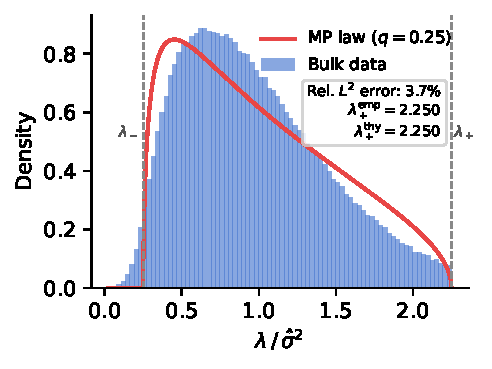
\includegraphics[width=1\columnwidth]{PETR4_M5_fig1_mp} \caption{Bulk eigenvalue density histogram of aggregated normalized bulk eigenvalues
across all windows for PETR4, M5 frequency. Orange curve: theoretical
MP density (Eq.~\ref{eq:MP}) with $q=0.25$, $\hat{\sigma}^{2}=1$.
Vertical dashed lines: theoretical $\lambda_{\pm}$. Inset: relative
$L^{2}$ error for all assets in Table~\ref{tab:assets}.}
\label{fig:mp_bulk} 
\end{figure}

\textbf{It� scaling ($\beta$).} Figure~\ref{fig:beta_alpha}(a)
shows the log-log plot of $\E[\|\Delta\K\|_{F}^{2}]$ vs.\ lag $\Delta\tau=\Delta\tau_{0}\cdot s$
for the diffusive regime, where $s\in\{1,2,4,8,16\}$. The slope $\beta\approx1$
is robust for both M5 and H1 data.

\begin{figure}
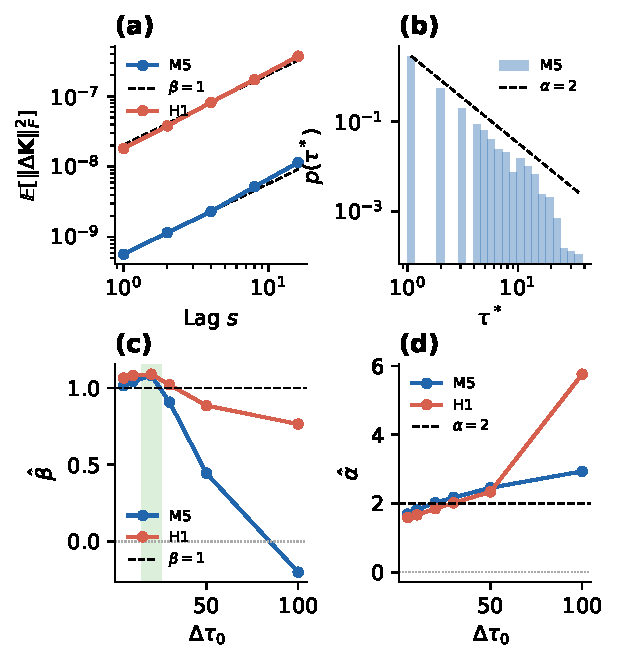
\includegraphics[width=1\columnwidth]{PETR4_fig2_exponents} \caption{Universal exponents, data from PETR4. (a) Log-log plot of $\E[\|\Delta\K\|_{F}^{2}]$
vs. temporal lag at M5 and H1 timescales. Dashed: slope $\beta=1$.
(b) Histogram of inter-regime intervals $\tau^{*}$ frequencies on
log-log scale for M5 timescale. Dashed: slope $\alpha=2$. (c) and
(d) Estimated $\beta$ (left) and $\alpha$ (right) as functions of
$\Delta\tau_{0}$(candles) for M5 and H1 timescales. Both exponents
converge to $(1,2)$ in the range $\Delta\tau_{0}\lesssim30$. The
shaded region is the optimal choice for observation step $\Delta\tau_{{\rm opt}}\approx20$.}
\label{fig:beta_alpha}
\end{figure}

\textbf{Inter-regime waiting times ($\alpha$).} Figure~\ref{fig:beta_alpha}(b)
shows the histogram of inter-regime intervals $\tau^{*}$ frequencies
on a log-log scale for PETR4 at M5. The Hill estimator gives $\alpha=????$
(mean $\pm$ std across assets), consistent with the theoretical prediction~\eqref{eq:alpha_prediction}.
Exponential or Gaussian waiting-time distributions, characteristic
of Poisson/GARCH regime models, are strongly rejected.

\textbf{Optimal observation step $\Delta\tau_{{\rm opt}}$.} Figure~\ref{fig:beta_alpha}(c)
shows $\beta$ as a function of observation step $\Delta\tau_{0}$,
with $L=80$ and $W=400$. A systematic maximum $\beta_{{\rm max}}$
at $\Delta\tau_{{\rm opt}}\approx20$ is observed for both M5 and
H1 frequencies.

\textbf{Optimal embedding dimension $L_{{\rm opt}}$.} Figure~\ref{fig:Lopt}
shows $\beta$ as a function of embedding dimension $L$, with $W=nL$
($n\in\{4,5,6\}$) held fixed to maintain constant $q$. A maximum
for diffusion exponent at $L_{{\rm opt}}\approx80$ is observed for
both M5 and H1 frequencies, a factor $12$ difference in physical
timescale, suggesting that $L_{{\rm opt}}$ measures an intrinsic
state-space dimension of the market, invariant under temporal rescaling.

\begin{figure}[t]
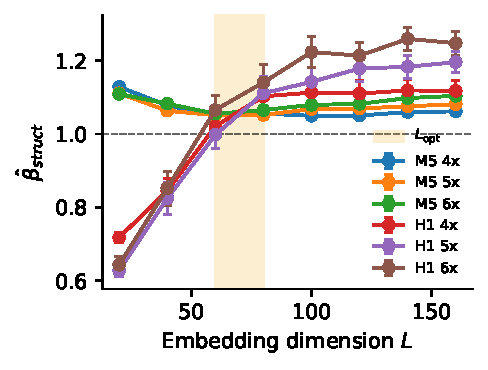
\includegraphics[width=1\columnwidth,height=0.35\textheight]{PETR4_fig3_Lopt}
\caption{Intrinsic embedding dimension. Diffusive exponent $\beta$ vs.\ embedding
dimension $L$ for M5 and H1 data, with $n=W/L\in\{4,5,6\}$. Both
timescales yield $L_{{\rm opt}}\approx80$ regardless of $n$. Shaded
region: $L_{{\rm opt}}\in[75,85]$. }
\label{fig:Lopt} 
\end{figure}

\textbf{Fluctuation--dissipation balance.} The ratio $R$ defined
in Eq.~\eqref{eq:ratio_R} satisfies $R=???$ across all assets and
frequencies within the diffusive regime, confirming the near-stationarity
of the Frobenius energy and the consistency of the It� description.

% ============================================================


\section{Discussion}

% ============================================================

The universality of $(\beta,\alpha)=(1,2)$ has strong theoretical
implications. $\beta=1$ implies that $\K(\tau)$ is Markovian at
the natural diffusive timescale: market memory is encoded in the instantaneous
state $\K(\tau)$, not in long-range correlations of the return series
itself. This is consistent with the observation that standard tests
for long memory in returns (Hurst exponent, DFA) yield ambiguous results~\cite{Beran1994},
the long-range structure resides in the operator dynamics, not in
scalar returns.

$\alpha=2$ identifies financial regime changes as belonging to the
universality class of critical point crossing by one-dimensional diffusions
with regular drift, the same class as certain interface depinning
transitions and record-breaking statistics \cite{Majumdar1999}. This
places financial timeseries within a well-understood class of physical
phenomena, offering a mechanistic explanation for the scale-free distribution
of crisis durations observed empirically.

$L_{{\rm opt}}\approx80$ independent of timescale suggests that markets
have an intrinsic finite-dimensional state space of $\sim80$ degrees
of freedom. One possible interpretation is that $L_{{\rm opt}}$ reflects
the effective dimensionality of market microstructure; whether it
scales with market complexity remains an open question.

The invariance of $\Delta\tau_{{\rm opt}}\approx20$ across timescales
suggests the existence of an intrinsic temporal coarse-graining scale
in market dynamics.

% ============================================================


\section{Conclusion}

% ============================================================

We have introduced a spectral framework for financial price dynamics
based on the It� evolution of the temporal covariance operator $\K(\tau)$.
The framework yields two analytically derived universal exponents
confirmed empirically across $13$ assets and four asset classes,
$\beta=1$ and $\alpha=2$. The MP law describes the bulk with relative
$L^{2}$ error below $4\%$, and an intrinsic embedding dimension
$L_{{\rm opt}}\approx80$ and observation step $\Delta\tau_{{\rm opt}}\approx20$
emerges independently of timescale. These results establish a direct
bridge between the physics of stochastic operators and the phenomenology
of financial markets.
\begin{acknowledgments}
We wold like to thank Prof. Eberth Correa for fruitful discussions.
\end{acknowledgments}

\bibliography{refs_natphys}

\end{document}
